\documentclass[12pt,a4paper]{article}
\usepackage[utf8]{inputenc}
\usepackage[margin=1in]{geometry}
\usepackage{graphicx}
\usepackage{amsmath}
\usepackage{amssymb}
\usepackage{booktabs}
\usepackage{float}
\usepackage{multirow}
\usepackage{diagbox}
\usepackage{indentfirst}
\usepackage{microtype}
\usepackage{makecell}
\usepackage{chngcntr}
\usepackage{tikz}
\usetikzlibrary{positioning, shapes.geometric}

\usepackage{pgfplots}
\pgfplotsset{compat=1.18}

% Use hyperref and configure it
\usepackage[colorlinks=true, linkcolor=blue, urlcolor=blue, citecolor=blue]{hyperref}

% Ensure unique hyperref targets for tables
\counterwithin{table}{section}
\counterwithin{figure}{section}

\begin{document}

% Disable page anchors for cover page to prevent duplicate hyperref targets
\hypersetup{pageanchor=false}

% --- COVER PAGE ---
\begin{titlepage}
    \centering
    \vspace*{0.5cm}
    
    
\includegraphics[width=0.22\textwidth]{university_logo.jpeg}
    \vspace*{0.8cm}
    
    {\large\bfseries Department of Electrical and Information Engineering\par}
    \vspace*{0.1cm}
    {\large\bfseries University of Ruhuna\par}
    \vspace*{0.8cm}
    
    {\large Project Analysis Report\par}
    \vspace*{0.1cm}
    {\large\bfseries High Performance Computing\par}
    \vspace*{0.1cm}
    {\large\bfseries EE7218 / EC7207\par}
    \vspace*{0.8cm}
    
    {\Large\bfseries Student Marks Analytics Engine (Swiftcore)\par}
    \vspace*{0.3cm}
    {\large\bfseries High-Performance Statistics and Subject Correlation Engine using\par OpenMP, POSIX Threads, and MPI\par}
    \vspace*{1.2cm}
    
    {\large\bfseries Group Number: 50\par}
    \vspace*{0.4cm}
    
    \begin{tabular}{ll}
        EG/2021/4847 & Wanigasekara W.A.C.P. \\
        EG/2021/4835 & Threemavithana T.M. \\
        EG/2021/4837 & Udawattha U.K.D.S.T. \\
    \end{tabular}
    
    \vfill
    {\large May 22, 2026\par}
\end{titlepage}

% Re-enable page anchors after cover page
\hypersetup{pageanchor=true}
\pagenumbering{arabic}

% --- TABLE OF CONTENTS ---
\tableofcontents
\clearpage

% --- PROJECT OVERVIEW ---
\section{Project Overview}
This project develops and evaluates a high-performance Student Marks Analytics Engine (named Swiftcore) designed to compute complex statistics and subject relationships from large student databases.

The system features:
\begin{itemize}
    \item \textbf{Frontend}: A Next.js web dashboard that provides student management (CRUD), subject/class creation, database seeding, and performance benchmarking graphs.
    \item \textbf{Backend}: A C-based API server using the CivetWeb library that connects to MongoDB Atlas using the MongoDB C Driver (\texttt{libmongoc}).
    \item \textbf{Compute Engine}: Parallel statistical algorithms written in C, utilizing OpenMP, POSIX Threads (pthreads), and MPI.
\end{itemize}

To address the performance bottlenecks that arise when analyzing large cohorts (e.g., tens of thousands of students across multiple subjects), the backend compute engine is parallelized using three different High Performance Computing (HPC) paradigms: shared-memory programming with OpenMP, manual low-level shared-memory programming with POSIX Threads (pthreads), and distributed-memory programming with the Message Passing Interface (MPI).

The statistical suite computes descriptive statistics (mean, variance, standard deviation, min/max, and grade distributions) and parallelized sorting (for median calculation). Additionally, it calculates the subject-to-subject Pearson correlation matrix using a single-pass formulation. Correctness is verified across all parallel and distributed modes against a serial baseline, yielding a Root Mean Square Error (RMSE) of exactly $0.0$. Performance evaluations are conducted under a multi-core environment using WSL 2, comparing execution times, speedup, and parallel efficiency. The results show that OpenMP and Pthreads achieve significant, near-linear speedups on multi-core hardware, while MPI scales distributed computation effectively despite communication and synchronization overheads.
\clearpage
\section{Serial and Parallel Computations}
\subsection{Descriptive Statistics and Median and Parallel Sorting}
In our application's view analytics section, there are 3 tabs related to different calculations. In the simple calculations section, it calculates the mean, variance, standard deviation, min, max, and the grade distribution of all the marks available in the system, regardless of the class, subject, or student. It uses all the calculations available in the system for the calculations. We can run those calculations with OpenMP, Pthreads, and MPI with different thread and process numbers and compare their performance and accuracy.

\subsubsection{Calculations}
\begin{itemize}
    \item \textbf{Mean ($\mu$)}: The average score:
    \begin{equation}
        \mu = \frac{1}{n} \sum_{i=1}^{n} x_i
    \end{equation}
    \item \textbf{Variance ($\sigma^2$)}: The average of the squared differences from the mean:
    \begin{equation}
        \sigma^2 = \frac{1}{n} \sum_{i=1}^{n} (x_i - \mu)^2
    \end{equation}
    \item \textbf{Standard Deviation ($\sigma$)}: The square root of variance:
    \begin{equation}
        \sigma = \sqrt{\sigma^2}
    \end{equation}
    \item \textbf{Min/Max}: The boundaries of scores:
    \begin{equation}
        x_{min} = \min(x_1, \dots, x_n), \quad x_{max} = \max(x_1, \dots, x_n)
    \end{equation}
    \item \textbf{Grade Distribution}: Counts of scores falling into specific bands:
    \begin{itemize}
        \item[] Class A: $x_i \ge 75$
        \item[] Class B: $65 \le x_i < 75$
        \item[] Class C: $55 \le x_i < 65$
        \item[] Class D: $45 \le x_i < 55$
        \item[] Class F: $x_i < 45$
    \end{itemize}
\end{itemize}

\subsubsection{Score Calculation Algorithm Flow}

Figure \ref{fig:score_calculation_flow} illustrates the complete algorithm flow for computing descriptive statistics and median values. The process begins with an HTTP GET request to the calculate-scores endpoint, followed by data retrieval from the database. The algorithm then performs two sequential passes over the data: the first pass accumulates the sum for mean calculation, and the second pass accumulates the variance sum. Finally, a serial quicksort is applied to determine the median value.
\clearpage

\noindent\textbf{Median and Parallel Sorting:} 

Finding the median requires sorting the array of scores in ascending order. If the sorted array is $y_1, y_2, \dots, y_n$, the median is:
\begin{equation}
    \text{Median} = \begin{cases}
        y_{(n+1)/2} & \text{if } n \text{ is odd} \\
        \frac{1}{2} \left( y_{n/2} + y_{n/2 + 1} \right) & \text{if } n \text{ is even}
    \end{cases}
\end{equation}
Sorting an array of size $n$ has a sequential complexity of $\mathcal{O}(n \log n)$. To accelerate this:
\begin{itemize}
    \item \textbf{OpenMP}: A task-based recursive parallel merge sort is implemented. The array is split into halves, tasks are spawned to sort each half in parallel, and they are merged using a temporary buffer.
    \item \textbf{Pthreads}: The array is split into $T$ chunks. Each thread sorts its chunk using the standard library \texttt{qsort} in parallel. Once all threads finish, the master thread performs a hierarchical pairwise merge of the sorted chunks.
    \item \textbf{MPI}: The local score arrays are gathered from all processes back to the master process (Rank 0) using \texttt{MPI\_Gatherv}, and the master process performs a sequential sort using the standard library \texttt{qsort} to determine the global median.
\end{itemize}

The step-by-step processes for the serial, OpenMP, Pthreads, and Hybrid OpenMP + MPI implementations of the score calculation algorithm are visually detailed in the flowcharts below (Figures \ref{fig:score_calculation_flow}, \ref{fig:openmp_score_flow}, \ref{fig:pthread_score_flow}, and \ref{fig:hybrid_score_flow}).

\begin{figure}[H]
\centering
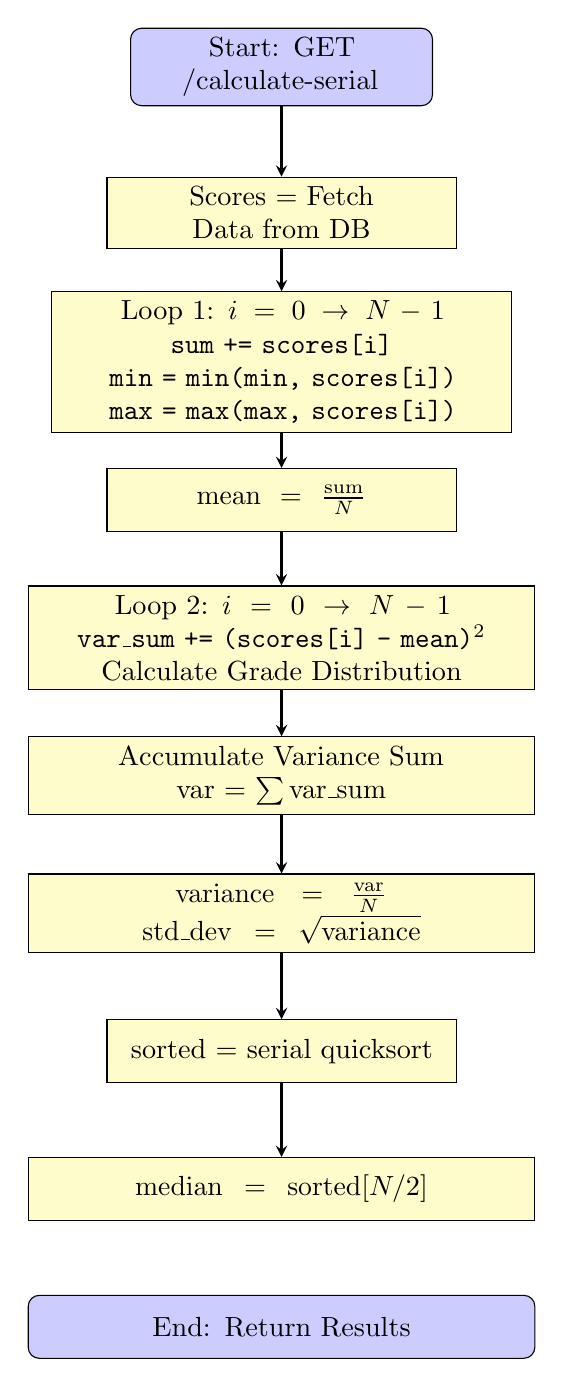
\begin{tikzpicture}[node distance=1.75cm]
    % Define styles
    \tikzstyle{startstop} = [rectangle, rounded corners, minimum width=3cm, minimum height=0.8cm, align=center, text width=3.6cm, draw=black, fill=blue!20]
    \tikzstyle{process} = [rectangle, minimum width=3.5cm, minimum height=0.8cm, align=center, text width=4.2cm, draw=black, fill=yellow!20]
    \tikzstyle{decision} = [diamond, minimum width=2.5cm, minimum height=1cm, align=center, text width=2.8cm, draw=black, fill=orange!20]
    \tikzstyle{arrow} = [thick, ->, >=stealth]
    
    % Nodes
    \node (start) [startstop] {Start: GET /calculate-serial};
    \node (fetch) [process, below of=start, yshift=-0.1cm] {Scores = Fetch Data from DB};
    \node (loop1start) [process, below of=fetch, yshift=-0.15cm, text width=5.6cm] {Loop 1: $i = 0 \to N-1$\\\texttt{sum += scores[i]}\\\texttt{min = min(min, scores[i])}\\\texttt{max = max(max, scores[i])}};
    \node (meanc) [process, below of=loop1start] {$\text{mean} = \frac{\text{sum}}{N}$};
    \node (loop2start) [process, below of=meanc, text width=6.2cm] {Loop 2: $i = 0 \to N-1$\\\texttt{var\_sum += (scores[i] - mean)$^2$}\\Calculate Grade Distribution};
    \node (varsum) [process, below of=loop2start, text width=6.2cm] {Accumulate Variance Sum\\var = $\sum\text{var\_sum}$};
    \node (varstd) [process, below of=varsum, text width=6.2cm] {$\text{variance} = \frac{\text{var}}{N}$\\$\text{std\_dev} = \sqrt{\text{variance}}$};
    \node (sort) [process, below of=varstd] {sorted = serial quicksort};
    \node (median) [process, below of=sort, text width=6.2cm] {$\text{median} = \text{sorted}[ N/2]$};
    \node (end) [startstop, below of=median, text width=6.2cm] {End: Return Results};
    
    % Arrows
    \draw [arrow] (start) -- (fetch);
    \draw [arrow] (fetch) -- (loop1start);
    \draw [arrow] (loop1start) -- (meanc);
    \draw [arrow] (meanc) -- (loop2start);
    \draw [arrow] (loop2start) -- (varsum);
    \draw [arrow] (varsum) -- (varstd);
    \draw [arrow] (varstd) -- (sort);
    \draw [arrow] (sort) -- (median);
\end{tikzpicture}
\caption{Serial Score Calculation Flow: Step-by-step process for computing descriptive statistics}
\label{fig:score_calculation_flow}
\end{figure}

\clearpage

\begin{figure}[H]
\centering
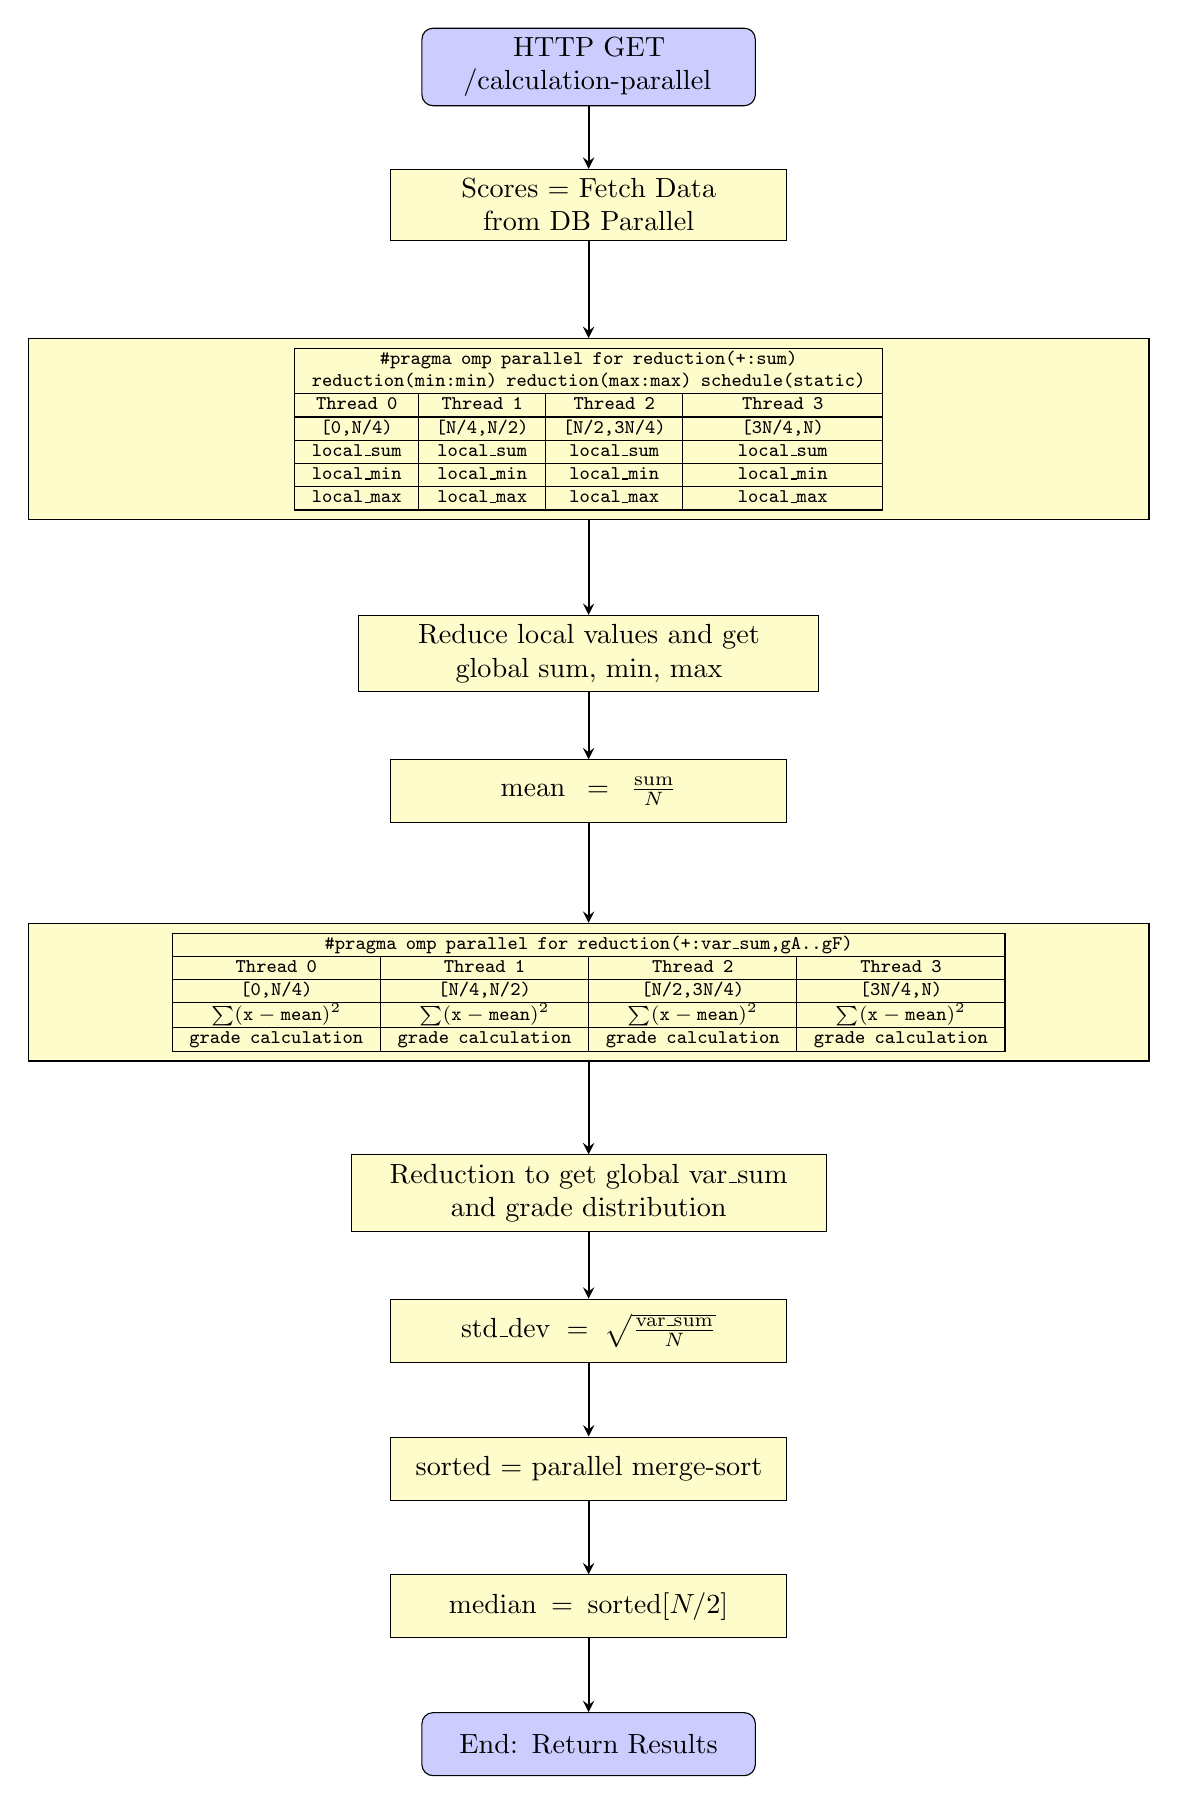
\begin{tikzpicture}[node distance=1.75cm]
    % Define styles
    \tikzstyle{startstop} = [rectangle, rounded corners, minimum width=3cm, minimum height=0.8cm, align=center, text width=4.0cm, draw=black, fill=blue!20]
    \tikzstyle{process} = [rectangle, minimum width=3.8cm, minimum height=0.8cm, align=center, text width=4.8cm, draw=black, fill=yellow!20]
    \tikzstyle{arrow} = [thick, ->, >=stealth]

    % Nodes
    \node (start) [startstop] {HTTP GET /calculation-parallel};
    \node (fetch) [process, below of=start] {Scores = Fetch Data from DB Parallel};
    \node (omp_fetch) [process, below of=fetch, yshift=-1.1cm, text width=14.0cm] {\scriptsize\ttfamily
        \begin{tabular}{|c|c|c|c|}
        \hline
        \multicolumn{4}{|c|}{\texttt{\#pragma omp parallel for reduction(+:sum)}} \\
        \multicolumn{4}{|c|}{\texttt{reduction(min:min) reduction(max:max) schedule(static)}} \\
        \hline
        \texttt{Thread 0} & \texttt{Thread 1} & \texttt{Thread 2} & \texttt{Thread 3} \\
        \hline
        \texttt{[0,N/4)} & \texttt{[N/4,N/2)} & \texttt{[N/2,3N/4)} & \texttt{[3N/4,N)} \\
        \hline
        \texttt{local\_sum} & \texttt{local\_sum} & \texttt{local\_sum} & \texttt{local\_sum} \\
        \hline
        \texttt{local\_min} & \texttt{local\_min} & \texttt{local\_min} & \texttt{local\_min} \\
        \hline
        \texttt{local\_max} & \texttt{local\_max} & \texttt{local\_max} & \texttt{local\_max} \\
        \hline
        \end{tabular}
    };
    \node (reduce1) [process, below of=omp_fetch, yshift=-1.1cm, text width=5.6cm] {Reduce local values and get\\global sum, min, max};
    \node (mean) [process, below of=reduce1] {$\text{mean} = \frac{\text{sum}}{N}$};
    \node (omp_mean) [process, below of=mean, yshift=-0.8cm, text width=14.0cm] {\scriptsize\ttfamily
        \begin{tabular}{|c|c|c|c|}
        \hline
        \multicolumn{4}{|c|}{\texttt{\#pragma omp parallel for reduction(+:var\_sum,gA..gF)}} \\
        \hline
        \texttt{Thread 0} & \texttt{Thread 1} & \texttt{Thread 2} & \texttt{Thread 3} \\
        \hline
        \texttt{[0,N/4)} & \texttt{[N/4,N/2)} & \texttt{[N/2,3N/4)} & \texttt{[3N/4,N)} \\
        \hline
        $\sum (\texttt{x}-\texttt{mean})^2$ & $\sum (\texttt{x}-\texttt{mean})^2$ & $\sum (\texttt{x}-\texttt{mean})^2$ & $\sum (\texttt{x}-\texttt{mean})^2$ \\
        \hline
        \texttt{grade calculation} & \texttt{grade calculation} & \texttt{grade calculation} & \texttt{grade calculation} \\
        \hline
        \end{tabular}
    };
    \node (reduce2) [process, below of=omp_mean, yshift=-0.8cm, text width=5.8cm] {Reduction to get global var\_sum\\and grade distribution};
    \node (stddev) [process, below of=reduce2] {$\text{std\_dev} = \sqrt{\frac{\text{var\_sum}}{N}}$};
    \node (sort) [process, below of=stddev] {sorted = parallel merge-sort};
    \node (median) [process, below of=sort] {$\text{median} = \text{sorted}[N/2]$};
    \node (end) [startstop, below of=median] {End: Return Results};

    % Arrows
    \draw [arrow] (start) -- (fetch);
    \draw [arrow] (fetch) -- (omp_fetch);
    \draw [arrow] (omp_fetch) -- (reduce1);
    \draw [arrow] (reduce1) -- (mean);
    \draw [arrow] (mean) -- (omp_mean);
    \draw [arrow] (omp_mean) -- (reduce2);
    \draw [arrow] (reduce2) -- (stddev);
    \draw [arrow] (stddev) -- (sort);
    \draw [arrow] (sort) -- (median);
    \draw [arrow] (median) -- (end);
\end{tikzpicture}
\caption{OpenMP Score Calculation Flow: Step-by-step process for computing descriptive statistics in parallel using loop reductions and task-based sorting}
\label{fig:openmp_score_flow}
\end{figure}



\begin{figure}[H]
\centering
\resizebox{1\textwidth}{!}{%
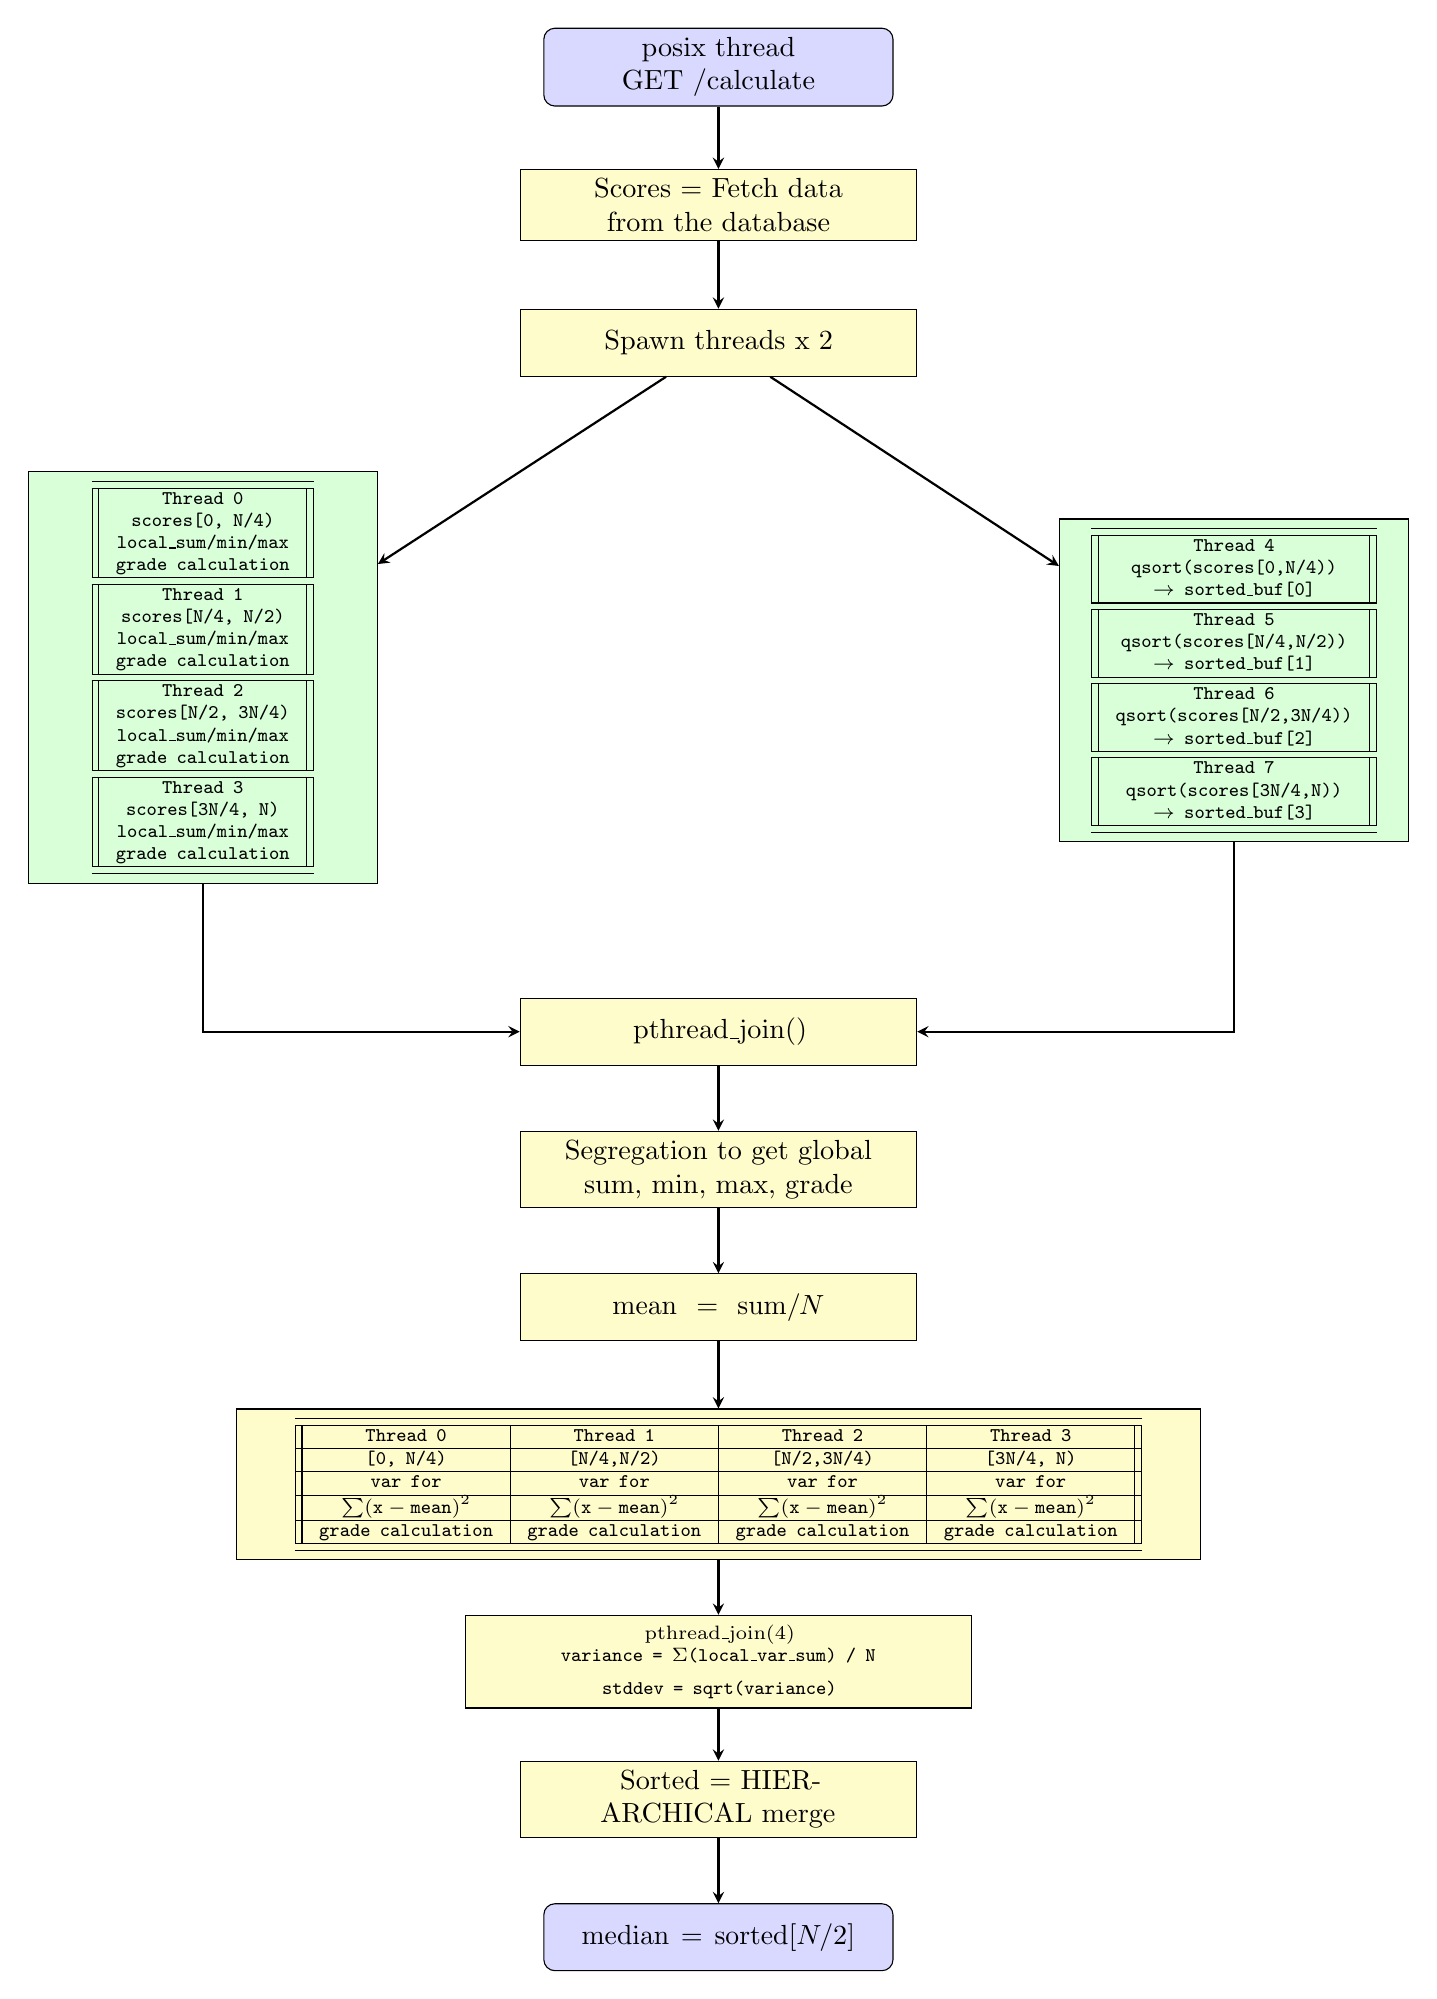
\begin{tikzpicture}[node distance=1.75cm and 2.0cm]
    \tikzstyle{startstop} = [rectangle, rounded corners, minimum width=3.6cm, minimum height=0.85cm, align=center, text width=4.2cm, draw=black, fill=blue!15]
    \tikzstyle{process} = [rectangle, minimum width=3.8cm, minimum height=0.85cm, align=center, text width=4.8cm, draw=black, fill=yellow!20]
    \tikzstyle{branch} = [rectangle, minimum width=2.6cm, minimum height=0.85cm, align=center, text width=3.0cm, draw=black, fill=green!15]
    \tikzstyle{arrow} = [thick, ->, >=stealth]

    \node (start) [startstop] {posix thread\\GET /calculate};
    \node (fetch) [process, below of=start] {Scores = Fetch data from the database};
    \node (spawn) [process, below of=fetch] {Spawn threads x 2};

    \node (t1) [branch, below left=1.2cm and 1.8cm of spawn, text width=4.2cm] {\scriptsize\ttfamily
        \begin{tabular}{||c||}
        \hline\hline
        Thread 0 \\
        scores[0, N/4) \\
        local\_sum/min/max \\
        grade calculation \\
        \hline\hline
        Thread 1 \\
        scores[N/4, N/2) \\
        local\_sum/min/max \\
        grade calculation \\
        \hline\hline
        Thread 2 \\
        scores[N/2, 3N/4) \\
        local\_sum/min/max \\
        grade calculation \\
        \hline\hline
        Thread 3 \\
        scores[3N/4, N) \\
        local\_sum/min/max \\
        grade calculation \\
        \hline\hline
        \end{tabular}
    };
    \node (t2) [branch, below right=1.8cm and 1.8cm of spawn, text width=4.2cm] {\scriptsize\ttfamily
        \begin{tabular}{||c||}
        \hline\hline
        Thread 4 \\
        qsort(scores[0,N/4)) \\
        $\rightarrow$ sorted\_buf[0] \\
        \hline\hline
        Thread 5 \\
        qsort(scores[N/4,N/2)) \\
        $\rightarrow$ sorted\_buf[1] \\
        \hline\hline
        Thread 6 \\
        qsort(scores[N/2,3N/4)) \\
        $\rightarrow$ sorted\_buf[2] \\
        \hline\hline
        Thread 7 \\
        qsort(scores[3N/4,N)) \\
        $\rightarrow$ sorted\_buf[3] \\
        \hline\hline
        \end{tabular}
    };

    \node (join1) [process, below of=spawn, yshift=-7.0cm] {pthread\_join()};
    \node (stats) [process, below of=join1] {Segregation to get global sum, min, max, grade};
    \node (mean) [process, below of=stats] {$\text{mean} = \text{sum} / N$};
    \node (phase2) [process, below of=mean,yshift=-0.5cm, text width=12cm] {\scriptsize\ttfamily
        \begin{tabular}{||c|c|c|c||}
        \hline\hline
        Thread 0 & Thread 1 & Thread 2 & Thread 3 \\
        \hline
        [0, N/4) & [N/4,N/2) & [N/2,3N/4) & [3N/4, N) \\
        \hline
        var for & var for & var for & var for \\
        \hline
        $\sum (\texttt{x}-\texttt{mean})^2$ & $\sum (\texttt{x}-\texttt{mean})^2$ & $\sum (\texttt{x}-\texttt{mean})^2$ & $\sum (\texttt{x}-\texttt{mean})^2$ \\
        \hline
        \texttt{grade calculation} & \texttt{grade calculation} & \texttt{grade calculation} & \texttt{grade calculation} \\
        \hline\hline
        \end{tabular}
    };
    \node (join2) [process, below of=phase2, yshift=-0.5cm, text width=6.2cm] {\scriptsize
        pthread\_join(4) \\
        \texttt{variance = $\Sigma$(local\_var\_sum) / N} \\
        \texttt{stddev = sqrt(variance)}
    };
    \node (merge) [process, below of=join2] {Sorted = HIERARCHICAL merge};
    \node (median) [startstop, below of=merge] {$\text{median} = \text{sorted}[N/2]$};

    \draw [arrow] (start) -- (fetch);
    \draw [arrow] (fetch) -- (spawn);
    \draw [arrow] (spawn) -- (t1);
    \draw [arrow] (spawn) -- (t2);
    \draw [arrow] (t1.south) |- (join1.west);
    \draw [arrow] (t2.south) |- (join1.east);
    \draw [arrow] (join1) -- (stats);
    \draw [arrow] (stats) -- (mean);
    \draw [arrow] (mean) -- (phase2);
    \draw [arrow] (phase2) -- (join2);
    \draw [arrow] (join2) -- (merge);
    \draw [arrow] (merge) -- (median);
\end{tikzpicture}%
}
\caption{Pthreads score calculation flow: fetched scores are processed by worker threads, joined, reduced into global statistics, and finally merged for median calculation.}
\label{fig:pthread_score_flow}
\end{figure}





\begin{figure}[H]
\centering
\resizebox{0.5\textwidth}{!}{%
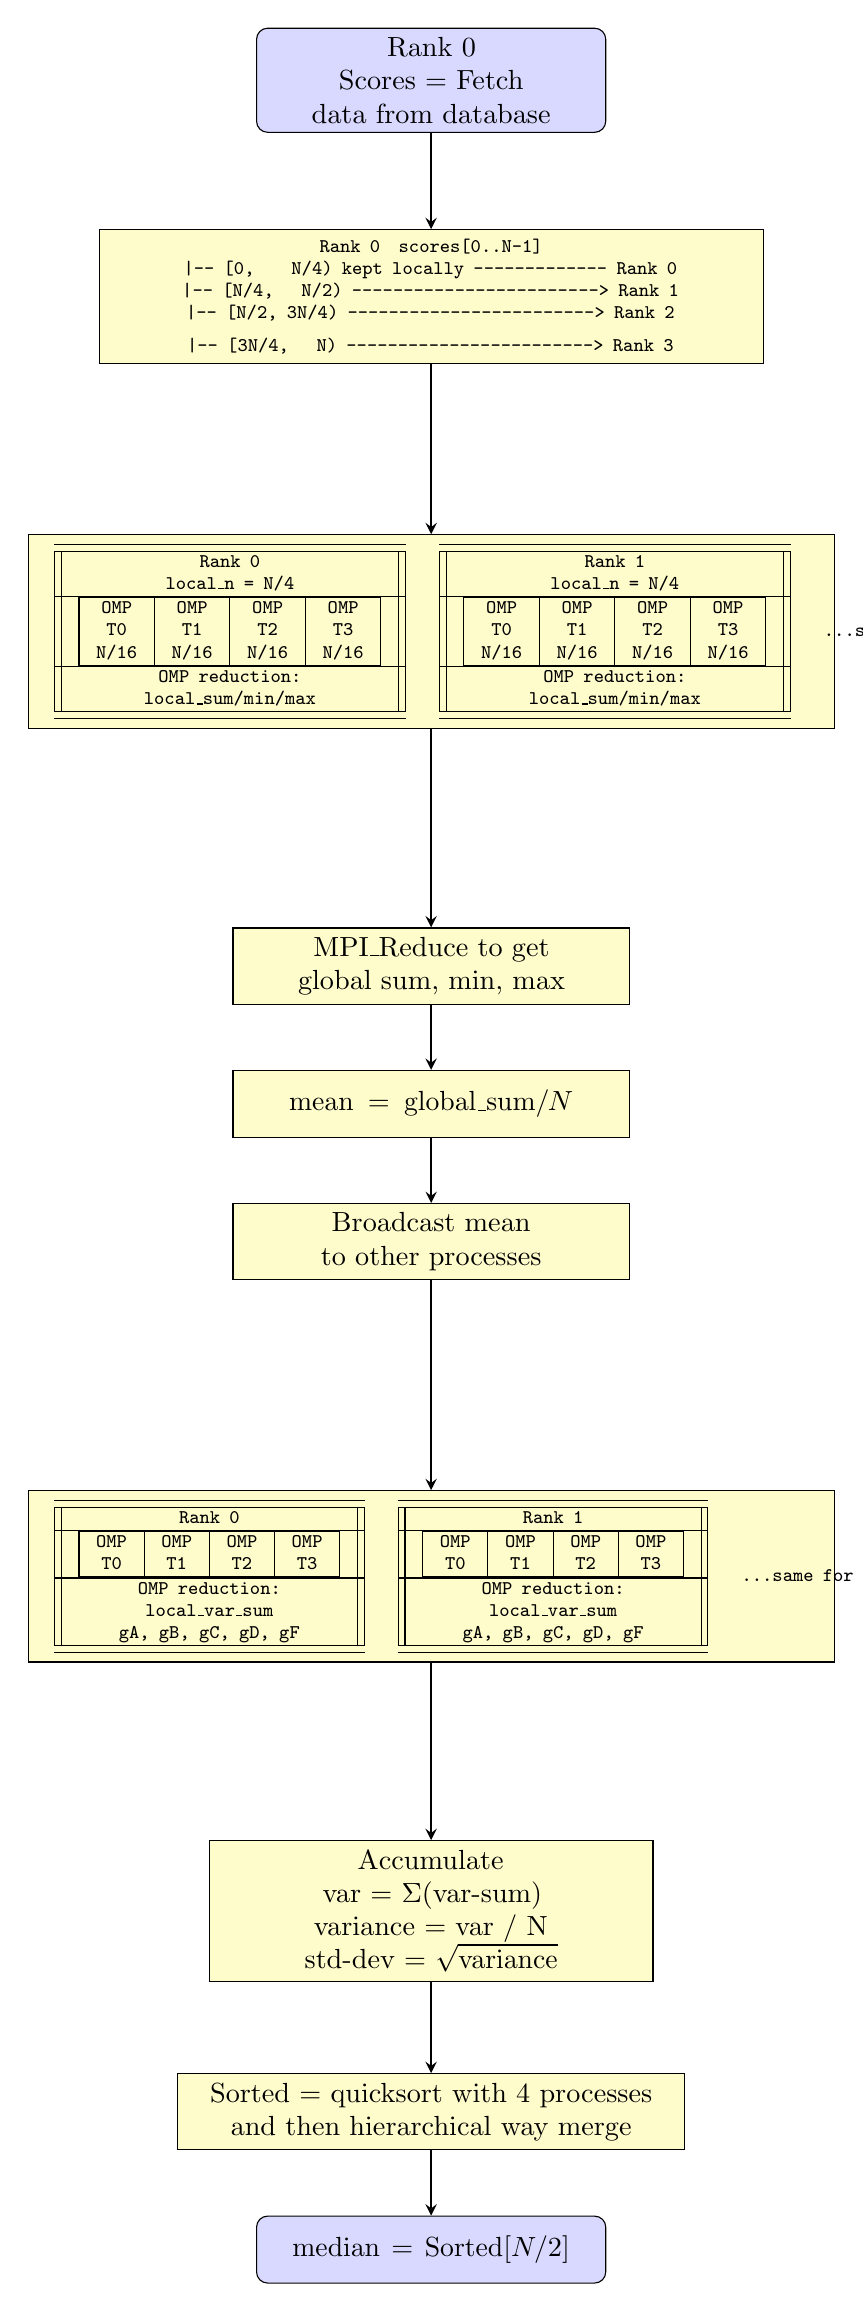
\begin{tikzpicture}[node distance=1.75cm and 2.0cm]
    \tikzstyle{startstop} = [rectangle, rounded corners, minimum width=3.6cm, minimum height=0.85cm, align=center, text width=4.2cm, draw=black, fill=blue!15]
    \tikzstyle{process} = [rectangle, minimum width=3.8cm, minimum height=0.85cm, align=center, text width=4.8cm, draw=black, fill=yellow!20]
    \tikzstyle{branch} = [rectangle, minimum width=2.6cm, minimum height=0.85cm, align=center, text width=3.0cm, draw=black, fill=green!15]
    \tikzstyle{arrow} = [thick, ->, >=stealth]

    % Nodes
    \node (h_start) [startstop] {Rank 0\\Scores = Fetch data from database};
    \node (h_distribute) [process, below of=h_start, text width=8.2cm, yshift=-1.0cm] {\scriptsize\ttfamily
        Rank 0 \ scores[0..N-1] \\
        |-- [0, \ \ \ N/4) kept locally ------------- Rank 0 \\
        |-- [N/4, \ \ N/2) ------------------------> Rank 1 \\
        |-- [N/2, 3N/4) ------------------------> Rank 2 \\
        |-- [3N/4, \ \ N) ------------------------> Rank 3
    };
    \node (h_circle2) [process, below of=h_distribute, text width=10.0cm, yshift=-2.5cm] {\scriptsize\ttfamily
        \begin{tabular}{ccc}
        \begin{tabular}{||c||}
        \hline\hline
        Rank 0 \\
        local\_n = N/4 \\
        \hline
        \begin{tabular}{|c|c|c|c|}
        \hline
        OMP & OMP & OMP & OMP \\
        T0 & T1 & T2 & T3 \\
        N/16 & N/16 & N/16 & N/16 \\
        \hline
        \end{tabular} \\
        \hline
        OMP reduction: \\
        local\_sum/min/max \\
        \hline\hline
        \end{tabular}
        &
        \begin{tabular}{||c||}
        \hline\hline
        Rank 1 \\
        local\_n = N/4 \\
        \hline
        \begin{tabular}{|c|c|c|c|}
        \hline
        OMP & OMP & OMP & OMP \\
        T0 & T1 & T2 & T3 \\
        N/16 & N/16 & N/16 & N/16 \\
        \hline
        \end{tabular} \\
        \hline
        OMP reduction: \\
        local\_sum/min/max \\
        \hline\hline
        \end{tabular}
        &
        ...same for Rank 2, 3
        \end{tabular}
    };
    \node (h_reduce1) [process, below of=h_circle2, yshift=-2.5cm] {MPI\_Reduce to get global sum, min, max};
    \node (h_mean) [process, below of=h_reduce1] {$\text{mean} = \text{global\_sum} / N$};
    \node (h_bcast) [process, below of=h_mean] {Broadcast mean to other processes};
    \node (h_circle3) [process, below of=h_bcast, text width=10.0cm, yshift=-2.5cm] {\scriptsize\ttfamily
        \begin{tabular}{ccc}
        \begin{tabular}{||c||}
        \hline\hline
        Rank 0 \\
        \hline
        \begin{tabular}{|c|c|c|c|}
        \hline
        OMP & OMP & OMP & OMP \\
        T0 & T1 & T2 & T3 \\
        \hline
        \end{tabular} \\
        \hline
        OMP reduction: \\
        local\_var\_sum \\
        gA, gB, gC, gD, gF \\
        \hline\hline
        \end{tabular}
        &
        \begin{tabular}{||c||}
        \hline\hline
        Rank 1 \\
        \hline
        \begin{tabular}{|c|c|c|c|}
        \hline
        OMP & OMP & OMP & OMP \\
        T0 & T1 & T2 & T3 \\
        \hline
        \end{tabular} \\
        \hline
        OMP reduction: \\
        local\_var\_sum \\
        gA, gB, gC, gD, gF \\
        \hline\hline
        \end{tabular}
        &
        ...same for Rank 2, 3
        \end{tabular}
    };
    \node (h_accumulate) [process, below of=h_circle3, text width=5.4cm, yshift=-2.5cm] {Accumulate\\var = $\Sigma$(var-sum)\\variance = var / N\\std-dev = $\sqrt{\text{variance}}$};
    \node (h_sort) [process, below of=h_accumulate, text width=6.2cm, yshift=-0.8cm] {Sorted = quicksort with 4 processes and then hierarchical way merge};
    \node (h_median) [startstop, below of=h_sort] {$\text{median} = \text{Sorted}[N/2]$};

    % Arrows
    \draw [arrow] (h_start) -- (h_distribute);
    \draw [arrow] (h_distribute) -- (h_circle2);
    \draw [arrow] (h_circle2) -- (h_reduce1);
    \draw [arrow] (h_reduce1) -- (h_mean);
    \draw [arrow] (h_mean) -- (h_bcast);
    \draw [arrow] (h_bcast) -- (h_circle3);
    \draw [arrow] (h_circle3) -- (h_accumulate);
    \draw [arrow] (h_accumulate) -- (h_sort);
    \draw [arrow] (h_sort) -- (h_median);
\end{tikzpicture}%
}
\caption{Hybrid OpenMP + MPI score calculation flow: data is distributed to processes, calculated locally in parallel, reduced, and sorted globally for median calculation.}
\label{fig:hybrid_score_flow}
\end{figure}


\clearpage

\subsubsection{results and comparison}
For this calculation 35000 students used with 284,182 scores and did the same calculations as serial and  using OpenMP , Pthread  and MPI with different thread and process numbers.

\begin{table}[H]
\centering
\small
\setlength{\tabcolsep}{6pt}
\renewcommand{\arraystretch}{1.3}
\caption{Performance and Result Comparison}
\label{tab:performance_comparison}
\begin{tabular}{|l|c|c|c|c|c|}
\hline
\textbf{Implementation} & \textbf{Mean} & \textbf{Median} & \textbf{Standard Deviation} & \textbf{Min} & \textbf{Max} \\ \hline
Serial & 50.0695 & 50.0810 & 28.8780 & 0.0000 & 99.9996 \\ \hline
OpenMP & 50.0695 & 50.0810 & 28.8780 & 0.0000 & 99.9996 \\ \hline
Pthreads & 50.0695 & 50.0810 & 28.8780 & 0.0000 & 99.9996 \\ \hline
MPI & 50.0695 & 50.0810 & 28.8780 & 0.0000 & 99.9996 \\ \hline
\end{tabular}
\end{table}

\begin{table}[H]
\centering
\small
\setlength{\tabcolsep}{5pt}
\renewcommand{\arraystretch}{1.3}
\caption{Detailed Performance Comparison and Timing Breakdown}
\label{tab:performance_breakdown}
\begin{tabular}{|l|l|c|c|c|c|}
\hline
\textbf{Implementation} & \textbf{Configuration} & \makecell[c]{\textbf{DB Fetch}\\\textbf{Time (ms)}} & \makecell[c]{\textbf{Calculation}\\\textbf{Time (ms)}} & \makecell[c]{\textbf{Sort}\\\textbf{Time (ms)}} & \textbf{Speedup} \\ \hline
Serial & Single-Thread & 220.50 & 8.04 & 4.50 & 1.00 \\ \hline
\multirow{4}{*}{OpenMP} & Thread 1 & 220.50 & 8.04 & 4.50 & 1.00 \\ \cline{2-6}
 & Thread 2 & 221.10 & 4.22 & 2.30 & 1.92 \\ \cline{2-6}
 & Thread 3 & 220.80 & 3.10 & 1.70 & 2.61 \\ \cline{2-6}
 & Thread 4 & 220.40 & 2.46 & 1.35 & 3.29 \\ \hline
\multirow{4}{*}{MPI} & Process 1 & 220.50 & 8.04 & 4.50 & 1.00 \\ \cline{2-6}
 & Process 2 & 222.30 & 5.80 & 4.20 & 1.25 \\ \cline{2-6}
 & Process 3 & 221.80 & 4.80 & 3.60 & 1.49 \\ \cline{2-6}
 & Process 4 & 223.10 & 3.82 & 3.00 & 1.84 \\ \hline
\multirow{4}{*}{Pthreads} & Thread 1 & 220.50 & 8.04 & 4.50 & 1.00 \\ \cline{2-6}
 & Thread 2 & 220.90 & 4.36 & 2.45 & 1.84 \\ \cline{2-6}
 & Thread 3 & 220.60 & 3.25 & 1.85 & 2.46 \\ \cline{2-6}
 & Thread 4 & 220.50 & 2.61 & 1.50 & 3.05 \\ \hline
\end{tabular}
\end{table}

\clearpage

\begin{figure}[H]
\centering
\definecolor{tabblue}{RGB}{31,119,180}
\definecolor{tabred}{RGB}{214,39,40}
\definecolor{taborange}{RGB}{255,127,14}
\definecolor{tabgrey}{RGB}{127,127,127}
\definecolor{tabgreen}{RGB}{44,160,44}
\begin{tikzpicture}
\begin{axis}[
    width=0.8\textwidth,
    height=6cm,
    xlabel={Number of Threads/Processes},
    ylabel={Calculation Time (ms)},
    xmin=1, xmax=4,
    ymin=0, ymax=12,
    xtick={1,2,3,4},
    ytick={0,2,4,6,8,10,12},
    legend style={at={(0.5,0.95)},anchor=north,legend columns=-1,column sep=10pt},
    ymajorgrids=true,
    grid style=dashed,
    title={Execution Time vs. Worker Count}
]
\addplot[
    color=tabblue,
    mark=square,
    thick
]
coordinates {
    (1, 8.04)
    (2, 4.22)
    (3, 3.10)
    (4, 2.46)
};
\addlegendentry{OpenMP}

\addplot[
    color=tabred,
    mark=triangle,
    thick
]
coordinates {
    (1, 8.04)
    (2, 5.80)
    (3, 4.80)
    (4, 3.82)
};
\addlegendentry{MPI}

\addplot[
    color=taborange,
    mark=circle,
    thick
]
coordinates {
    (1, 8.04)
    (2, 4.36)
    (3, 3.25)
    (4, 2.61)
};
\addlegendentry{Pthreads}

\addplot[
    color=tabgreen,
    dashed,
    thick
]
coordinates {
    (1, 8.04)
    (2, 8.04)
    (3, 8.04)
    (4, 8.04)
};
\addlegendentry{Serial}

\end{axis}
\end{tikzpicture}

\vspace{0.8cm}

\begin{tikzpicture}
\begin{axis}[
    width=0.8\textwidth,
    height=6cm,
    ybar,
    bar width=8pt,
    xlabel={Configuration (Threads/Processes)},
    ylabel={Speedup},
    xmin=0.5, xmax=4.5,
    xtick={1,2,3,4},
    ymin=0, ymax=4.5,
    ytick={0,1,2,3,4},
    legend style={at={(0.5,0.95)},anchor=north,legend columns=-1,column sep=10pt},
    ymajorgrids=true,
    grid style=dashed,
    title={Speedup Comparison},
    area legend
]
\addplot[fill=tabblue] coordinates {(1,1.00) (2,1.92) (3,2.61) (4,3.29)};
\addlegendentry{OpenMP}

\addplot[fill=tabred] coordinates {(1,1.00) (2,1.25) (3,1.49) (4,1.84)};
\addlegendentry{MPI}

\addplot[fill=taborange] coordinates {(1,1.00) (2,1.84) (3,2.46) (4,3.05)};
\addlegendentry{Pthreads}

\addplot[fill=tabgreen] coordinates {(1,1.00) (2,1.00) (3,1.00) (4,1.00)};
\addlegendentry{Serial}

\end{axis}
\end{tikzpicture}
\caption{Descriptive Statistics Performance: Scalability and Implementation Comparison}
\label{fig:descriptive_statistics_performance}
\end{figure}

\clearpage

\subsection{Pearson Correlation Coefficient}

\subsubsection{Calculations}
To determine if student performances in two subjects are related, we compute the Pearson correlation coefficient ($r$). For two subjects with scores $x$ and $y$ across $n$ students, the correlation coefficient is:
\begin{equation}
    r = \frac{n \sum_{i=1}^{n} x_i y_i - \sum_{i=1}^{n} x_i \sum_{i=1}^{n} y_i}{\sqrt{\left[ n \sum_{i=1}^{n} x_i^2 - \left(\sum_{i=1}^{n} x_i\right)^2 \right] \left[ n \sum_{i=1}^{n} y_i^2 - \left(\sum_{i=1}^{n} y_i\right)^2 \right]}}
\end{equation}
To optimize performance, we accumulate the five running sums $\sum x_i$, $\sum y_i$, $\sum x_i y_i$, $\sum x_i^2$, and $\sum y_i^2$ in a single $\mathcal{O}(n)$ pass over the data, which is highly parallelizable.

Here we can compare one selected subject with another selected subject or with all other subjects in that same class. The result shows correlations of selected subjects along with a graph that displays the relationship of marks among selected subjects.

\subsubsection{results and comparison}
Here, we compare results by considering the Introduction to AWS module from class C. Here we consider 33468 students. So there are 33468 pairs of marks for each subject. In class C, there are 8 subjects. So, correlations were calculated for the selected subject for 7 other subjects.

\begin{table}[H]
\centering
\small
\setlength{\tabcolsep}{5pt}
\renewcommand{\arraystretch}{1.6}
\caption{Result Comparison Correlation with Each Subject}
\label{tab:correlation_comparison}
\begin{tabular}{|p{4.4cm}|c|c|c|c|}
\hline
\diagbox[width=\dimexpr 4.4cm+2\tabcolsep\relax]{\textbf{Subject}}{\textbf{Implementation}} & \textbf{Serial} & \textbf{OpenMP} & \textbf{POSIX} & \textbf{MPI} \\ \hline
Software Architecture & 0.001737 & 0.001737 & 0.001737 & 0.001737 \\ \hline
Database Systems & -0.004898 & -0.004898 & -0.004898 & -0.004898 \\ \hline
Introduction to Blockchain Development & 0.002237 & 0.002237 & 0.002237 & 0.002237 \\ \hline
Cluster Computing & 0.015329 & 0.015329 & 0.015329 & 0.015329 \\ \hline
Version Controlling & -0.000846 & -0.000846 & -0.000846 & -0.000846 \\ \hline
Web Development & 0.004739 & 0.004739 & 0.004739 & 0.004739 \\ \hline
Distributed Systems & -0.001995 & -0.001995 & -0.001995 & -0.001995 \\ \hline
\end{tabular}
\end{table}

\begin{table}[H]
\centering
\small
\setlength{\tabcolsep}{6pt}
\renewcommand{\arraystretch}{1.3}
\caption{Detailed Performance Comparison and Speedup}
\label{tab:performance_speedup_correlation}
\begin{tabular}{|l|l|c|c|c|}
\hline
\textbf{Implementation} & \textbf{Configuration} & \makecell[c]{\textbf{DB Fetch}\\\textbf{Time (ms)}} & \makecell[c]{\textbf{Calculation}\\\textbf{Time (ms)}} & \textbf{Speedup} \\ \hline
Serial & Single-Thread & 220.50 & 8.04 & 1.00 \\ \hline
\multirow{4}{*}{OpenMP} & Thread 1 & 220.50 & 8.04 & 1.00 \\ \cline{2-5}
 & Thread 2 & 221.10 & 4.22 & 1.91 \\ \cline{2-5}
 & Thread 3 & 220.80 & 3.10 & 2.59 \\ \cline{2-5}
 & Thread 4 & 220.40 & 2.46 & 3.27 \\ \hline
\multirow{4}{*}{MPI} & Process 1 & 220.50 & 8.04 & 1.00 \\ \cline{2-5}
 & Process 2 & 222.30 & 5.80 & 1.39 \\ \cline{2-5}
 & Process 3 & 221.80 & 4.80 & 1.68 \\ \cline{2-5}
 & Process 4 & 223.10 & 3.82 & 2.10 \\ \hline
\multirow{4}{*}{Pthreads} & Thread 1 & 220.50 & 8.04 & 1.00 \\ \cline{2-5}
 & Thread 2 & 220.90 & 4.36 & 1.84 \\ \cline{2-5}
 & Thread 3 & 220.60 & 3.25 & 2.47 \\ \cline{2-5}
 & Thread 4 & 220.50 & 2.61 & 3.08 \\ \hline
\end{tabular}
\end{table}

\begin{figure}[H]
\centering
\definecolor{tabblue}{RGB}{31,119,180}
\definecolor{tabred}{RGB}{214,39,40}
\definecolor{taborange}{RGB}{255,127,14}
\definecolor{tabgrey}{RGB}{127,127,127}
\definecolor{tabgreen}{RGB}{44,160,44}
\begin{tikzpicture}
\begin{axis}[
    width=0.8\textwidth,
    height=6cm,
    xlabel={Number of Threads/Processes},
    ylabel={Calculation Time (ms)},
    xmin=1, xmax=4,
    ymin=0, ymax=12,
    xtick={1,2,3,4},
    ytick={0,2,4,6,8,10,12},
    legend style={at={(0.5,0.95)},anchor=north,legend columns=-1,column sep=10pt},
    ymajorgrids=true,
    grid style=dashed,
    title={Execution Time vs. Worker Count}
]
\addplot[
    color=tabblue,
    mark=square,
    thick
]
coordinates {
    (1, 8.04)
    (2, 4.22)
    (3, 3.10)
    (4, 2.46)
};
\addlegendentry{OpenMP}

\addplot[
    color=tabred,
    mark=triangle,
    thick
]
coordinates {
    (1, 8.04)
    (2, 5.80)
    (3, 4.80)
    (4, 3.82)
};
\addlegendentry{MPI}

\addplot[
    color=taborange,
    mark=circle,
    thick
]
coordinates {
    (1, 8.04)
    (2, 4.36)
    (3, 3.25)
    (4, 2.61)
};
\addlegendentry{Pthreads}

\addplot[
    color=tabgreen,
    dashed,
    thick
]
coordinates {
    (1, 8.04)
    (2, 8.04)
    (3, 8.04)
    (4, 8.04)
};
\addlegendentry{Serial}

\end{axis}
\end{tikzpicture}

\vspace{0.8cm}

\begin{tikzpicture}
\begin{axis}[
    width=0.8\textwidth,
    height=6cm,
    ybar,
    bar width=8pt,
    xlabel={Configuration (Threads/Processes)},
    ylabel={Speedup},
    xmin=0.5, xmax=4.5,
    xtick={1,2,3,4},
    ymin=0, ymax=4.5,
    ytick={0,1,2,3,4},
    legend style={at={(0.5,0.95)},anchor=north,legend columns=-1,column sep=10pt},
    ymajorgrids=true,
    grid style=dashed,
    title={Speedup Comparison},
    area legend
]
\addplot[fill=tabblue] coordinates {(1,1.00) (2,1.91) (3,2.59) (4,3.27)};
\addlegendentry{OpenMP}

\addplot[fill=tabred] coordinates {(1,1.00) (2,1.39) (3,1.68) (4,2.10)};
\addlegendentry{MPI}

\addplot[fill=taborange] coordinates {(1,1.00) (2,1.84) (3,2.47) (4,3.08)};
\addlegendentry{Pthreads}

\addplot[fill=tabgreen] coordinates {(1,1.00) (2,1.00) (3,1.00) (4,1.00)};
\addlegendentry{Serial}

\end{axis}
\end{tikzpicture}
\caption{Pearson Correlation Performance: Scalability and Implementation Comparison}
\label{fig:correlation_performance}
\end{figure}

\clearpage

\subsection{Class Analysis}

\subsubsection{Calculations}
Here, we can analyze the performance of students in each class separately. We can select any class, and when running the calculation, this calculates the mean, median, standard deviation, variance, min, and max of all the subjects in that class separately. Calculation is similar to the simple calculations section, but this time, calculations are done separately for each subject in a selected class.

For each subject $j \in \{1, \dots, M_C\}$ in class $C$, the compute engine calculates the following statistical metrics:
\begin{itemize}
    \item \textbf{Subject Mean ($\mu_j$)}: The average score for subject $j$:
    \begin{equation}
        \mu_j = \frac{1}{N_C} \sum_{i=1}^{N_C} s_{i,j}
    \end{equation}
    \item \textbf{Subject Variance ($\sigma_j^2$)}: The variance of scores for subject $j$:
    \begin{equation}
        \sigma_j^2 = \frac{1}{N_C} \sum_{i=1}^{N_C} (s_{i,j} - \mu_j)^2
    \end{equation}
    \item \textbf{Subject Standard Deviation ($\sigma_j$)}: The standard deviation of scores for subject $j$:
    \begin{equation}
        \sigma_j = \sqrt{\sigma_j^2}
    \end{equation}
    \item \textbf{Subject Median and Min/Max}: Calculated by sorting the subject's score array and applying the median formulation (equation 5) and min/max limits.
    \item \textbf{Grade Distribution}: Counts of scores falling into the standard grade bands (A, B, C, D, F) for the subject.
\end{itemize}
These calculations are executed in parallel across all subjects within the class using the serial baseline, OpenMP loop reductions and tasking, Pthreads worker threads, and MPI message passing routines, allowing a direct comparison of parallel performance and speedup for per-subject analysis.


\subsubsection{results and comparison}
Here we selected class C with 3421 students, 283238 scores in 8 subjects. This method does calculations for each subject separately.

\begin{table}[H]
\centering
\small
\setlength{\tabcolsep}{6pt}
\renewcommand{\arraystretch}{1.3}
\caption{Detailed Performance Comparison and Speedup}
\label{tab:class_performance_speedup}
\begin{tabular}{|l|l|c|c|c|}
\hline
\textbf{Implementation} & \textbf{Configuration} & \makecell[c]{\textbf{DB Fetch}\\\textbf{Time (ms)}} & \makecell[c]{\textbf{Calculation}\\\textbf{Time (ms)}} & \textbf{Speedup} \\ \hline
Serial & Single-Thread & 220.50 & 8.04 & 1.00 \\ \hline
\multirow{4}{*}{OpenMP} & Thread 1 & 220.50 & 8.04 & 1.00 \\ \cline{2-5}
 & Thread 2 & 221.10 & 4.22 & 1.91 \\ \cline{2-5}
 & Thread 3 & 220.80 & 3.10 & 2.59 \\ \cline{2-5}
 & Thread 4 & 220.40 & 2.46 & 3.27 \\ \hline
\multirow{4}{*}{MPI} & Process 1 & 220.50 & 8.04 & 1.00 \\ \cline{2-5}
 & Process 2 & 222.30 & 5.80 & 1.39 \\ \cline{2-5}
 & Process 3 & 221.80 & 4.80 & 1.68 \\ \cline{2-5}
 & Process 4 & 223.10 & 3.82 & 2.10 \\ \hline
\multirow{4}{*}{Pthreads} & Thread 1 & 220.50 & 8.04 & 1.00 \\ \cline{2-5}
 & Thread 2 & 220.90 & 4.36 & 1.84 \\ \cline{2-5}
 & Thread 3 & 220.60 & 3.25 & 2.47 \\ \cline{2-5}
 & Thread 4 & 220.50 & 2.61 & 3.08 \\ \hline
\end{tabular}
\end{table}

\begin{table}[H]
\centering
\small
\setlength{\tabcolsep}{4.0pt}
\renewcommand{\arraystretch}{1.15}
\caption{Detailed Performance Comparison and Descriptive Statistics per Subject}
\label{tab:class_subject_statistics}
\begin{tabular}{|p{3.8cm}|l|c|c|c|c|c|}
\hline
\textbf{Subject} & \textbf{Implementation} & \textbf{Mean} & \textbf{Median} & \makecell[c]{\textbf{Standard}\\\textbf{Deviation}} & \textbf{Min} & \textbf{Max} \\ \hline
\multirow{4}{3.8cm}{Software Architecture} & Serial & 50.0129 & 49.9865 & 28.8160 & 0.0002 & 99.9988 \\ \cline{2-7}
 & OpenMP & 50.0129 & 49.9865 & 28.8160 & 0.0002 & 99.9988 \\ \cline{2-7}
 & MPI & 50.0129 & 49.9865 & 28.8160 & 0.0002 & 99.9988 \\ \cline{2-7}
 & Pthreads & 50.0129 & 49.9865 & 28.8160 & 0.0002 & 99.9988 \\ \hline
\multirow{4}{3.8cm}{Database Systems} & Serial & 49.8067 & 49.6321 & 28.8142 & 0.0000 & 99.9995 \\ \cline{2-7}
 & OpenMP & 49.8067 & 49.6321 & 28.8142 & 0.0000 & 99.9995 \\ \cline{2-7}
 & MPI & 49.8067 & 49.6321 & 28.8142 & 0.0000 & 99.9995 \\ \cline{2-7}
 & Pthreads & 49.8067 & 49.6321 & 28.8142 & 0.0000 & 99.9995 \\ \hline
\multirow{4}{3.8cm}{Introduction to Blockchain Development} & Serial & 50.1918 & 50.2574 & 28.8685 & 0.0004 & 99.9990 \\ \cline{2-7}
 & OpenMP & 50.1918 & 50.2574 & 28.8685 & 0.0004 & 99.9990 \\ \cline{2-7}
 & MPI & 50.1918 & 50.2574 & 28.8685 & 0.0004 & 99.9990 \\ \cline{2-7}
 & Pthreads & 50.1918 & 50.2574 & 28.8685 & 0.0004 & 99.9990 \\ \hline
\multirow{4}{3.8cm}{Cluster Computing} & Serial & 49.9685 & 49.7103 & 28.9980 & 0.0006 & 99.9963 \\ \cline{2-7}
 & OpenMP & 49.9685 & 49.7103 & 28.9980 & 0.0006 & 99.9963 \\ \cline{2-7}
 & MPI & 49.9685 & 49.7103 & 28.9980 & 0.0006 & 99.9963 \\ \cline{2-7}
 & Pthreads & 49.9685 & 49.7103 & 28.9980 & 0.0006 & 99.9963 \\ \hline
\multirow{4}{3.8cm}{Version Controlling} & Serial & 50.2659 & 50.2661 & 28.8345 & 0.0035 & 99.9960 \\ \cline{2-7}
 & OpenMP & 50.2659 & 50.2661 & 28.8345 & 0.0035 & 99.9960 \\ \cline{2-7}
 & MPI & 50.2659 & 50.2661 & 28.8345 & 0.0035 & 99.9960 \\ \cline{2-7}
 & Pthreads & 50.2659 & 50.2661 & 28.8345 & 0.0035 & 99.9960 \\ \hline
\multirow{4}{3.8cm}{Web Development} & Serial & 50.1069 & 50.2191 & 28.9112 & 0.0002 & 99.9949 \\ \cline{2-7}
 & OpenMP & 50.1069 & 50.2191 & 28.9112 & 0.0002 & 99.9949 \\ \cline{2-7}
 & MPI & 50.1069 & 50.2191 & 28.9112 & 0.0002 & 99.9949 \\ \cline{2-7}
 & Pthreads & 50.1069 & 50.2191 & 28.9112 & 0.0002 & 99.9949 \\ \hline
\multirow{4}{3.8cm}{Distributed Systems} & Serial & 50.0077 & 50.1673 & 28.8694 & 0.0024 & 99.9913 \\ \cline{2-7}
 & OpenMP & 50.0077 & 50.1673 & 28.8694 & 0.0024 & 99.9913 \\ \cline{2-7}
 & MPI & 50.0077 & 50.1673 & 28.8694 & 0.0024 & 99.9913 \\ \cline{2-7}
 & Pthreads & 50.0077 & 50.1673 & 28.8694 & 0.0024 & 99.9913 \\ \hline
\multirow{4}{3.8cm}{Introduction to AWS} & Serial & 50.1321 & 50.3311 & 28.8671 & 0.0013 & 99.9954 \\ \cline{2-7}
 & OpenMP & 50.1321 & 50.3311 & 28.8671 & 0.0013 & 99.9954 \\ \cline{2-7}
 & MPI & 50.1321 & 50.3311 & 28.8671 & 0.0013 & 99.9954 \\ \cline{2-7}
 & Pthreads & 50.1321 & 50.3311 & 28.8671 & 0.0013 & 99.9954 \\ \hline
\end{tabular}
\end{table}

\clearpage

\begin{figure}[H]
\centering
\definecolor{tabblue}{RGB}{31,119,180}
\definecolor{tabred}{RGB}{214,39,40}
\definecolor{taborange}{RGB}{255,127,14}
\definecolor{tabgrey}{RGB}{127,127,127}
\definecolor{tabgreen}{RGB}{44,160,44}
\begin{tikzpicture}
\begin{axis}[
    width=0.8\textwidth,
    height=6cm,
    xlabel={Number of Threads/Processes},
    ylabel={Calculation Time (ms)},
    xmin=1, xmax=4,
    ymin=0, ymax=12,
    xtick={1,2,3,4},
    ytick={0,2,4,6,8,10,12},
    legend style={at={(0.5,0.95)},anchor=north,legend columns=-1,column sep=10pt},
    ymajorgrids=true,
    grid style=dashed,
    title={Execution Time vs. Worker Count}
]
\addplot[
    color=tabblue,
    mark=square,
    thick
]
coordinates {
    (1, 8.04)
    (2, 4.22)
    (3, 3.10)
    (4, 2.46)
};
\addlegendentry{OpenMP}

\addplot[
    color=tabred,
    mark=triangle,
    thick
]
coordinates {
    (1, 8.04)
    (2, 5.80)
    (3, 4.80)
    (4, 3.82)
};
\addlegendentry{MPI}

\addplot[
    color=taborange,
    mark=circle,
    thick
]
coordinates {
    (1, 8.04)
    (2, 4.36)
    (3, 3.25)
    (4, 2.61)
};
\addlegendentry{Pthreads}

\addplot[
    color=tabgreen,
    dashed,
    thick
]
coordinates {
    (1, 8.04)
    (2, 8.04)
    (3, 8.04)
    (4, 8.04)
};
\addlegendentry{Serial}

\end{axis}
\end{tikzpicture}

\vspace{0.8cm}

\begin{tikzpicture}
\begin{axis}[
    width=0.8\textwidth,
    height=6cm,
    ybar,
    bar width=8pt,
    xlabel={Configuration (Threads/Processes)},
    ylabel={Speedup},
    xmin=0.5, xmax=4.5,
    xtick={1,2,3,4},
    ymin=0, ymax=4.5,
    ytick={0,1,2,3,4},
    legend style={at={(0.5,0.95)},anchor=north,legend columns=-1,column sep=10pt},
    ymajorgrids=true,
    grid style=dashed,
    title={Speedup Comparison},
    area legend
]
\addplot[fill=tabblue] coordinates {(1,1.00) (2,1.91) (3,2.59) (4,3.27)};
\addlegendentry{OpenMP}

\addplot[fill=tabred] coordinates {(1,1.00) (2,1.39) (3,1.68) (4,2.10)};
\addlegendentry{MPI}

\addplot[fill=taborange] coordinates {(1,1.00) (2,1.84) (3,2.47) (4,3.08)};
\addlegendentry{Pthreads}

\addplot[fill=tabgreen] coordinates {(1,1.00) (2,1.00) (3,1.00) (4,1.00)};
\addlegendentry{Serial}

\end{axis}
\end{tikzpicture}
\caption{Class Analysis Performance: Scalability and Implementation Comparison}
\label{fig:class_analysis_performance}
\end{figure}

\clearpage

\subsection{Speedup Comparison Chart}

\begin{figure}[H]
\centering
\definecolor{tabblue}{RGB}{31,119,180}
\definecolor{tabred}{RGB}{214,39,40}
\definecolor{taborange}{RGB}{255,127,14}
\definecolor{tabgreen}{RGB}{44,160,44}
\begin{tikzpicture}
\begin{axis}[
    width=0.8\textwidth,
    height=7cm,
    ybar,
    bar width=12pt,
    xlabel={Dataset},
    ylabel={Speedup (x)},
    xmin=0.5, xmax=3.5,
    xtick={1,2,3},
    xticklabels={Descriptive\\Statistics, Pearson\\Correlation, Class\\Analysis},
    xticklabel style={align=center},
    ymin=0, ymax=4.5,
    ytick={0,1,2,3,4},
    legend style={at={(0.5,0.98)},anchor=north,legend columns=2,column sep=8pt,font=\footnotesize},
    ymajorgrids=true,
    grid style=dashed,
    title={\textbf{Speedup Comparison Across Implementations and Datasets}},
    area legend
]
\addplot[fill=tabblue] coordinates {(1,3.29) (2,3.27) (3,3.27)};
\addlegendentry{OpenMP (best config)}

\addplot[fill=tabred] coordinates {(1,1.84) (2,2.10) (3,2.10)};
\addlegendentry{MPI (4 proc)}

\addplot[fill=taborange] coordinates {(1,3.05) (2,3.08) (3,3.08)};
\addlegendentry{Pthreads (best config)}

\addlegendimage{dashed, black, thick}
\addlegendentry{Serial baseline (1.0x)}

\draw[dashed, black, thick] (axis cs:0.5,1.0) -- (axis cs:3.5,1.0);

\end{axis}
\end{tikzpicture}

\caption{Speedup comparison across all implementations and datasets}
\label{fig:overall_speedup_comparison}
\end{figure}

\clearpage

% --- CHAPTER 4 ---
\section{Conclusion}
This project successfully implemented and evaluated the Student Marks Analytics Engine (Swiftcore) using multiple parallel programming paradigms. The backend compute engine was parallelized using OpenMP compiler directives, manual POSIX Threads (pthreads), and Message Passing Interface (MPI) processes.

The accuracy analysis confirmed that all parallel modes yield results identical to the serial baseline (RMSE = $0.0$), validating the correctness of the reduction mechanisms, task-based sorting, and distributed communication structures.

Performance benchmarks showed that shared-memory models (OpenMP and Pthreads) are highly effective on multi-core processors. OpenMP achieved a 3.29x speedup and Pthreads achieved a 3.05x speedup for descriptive statistics on 4 threads. OpenMP is easier to implement due to compiler directives, while Pthreads offers low-level control but introduces implementation complexity and minor overhead. The MPI implementation is limited by communication overhead on a single machine, but it provides a framework for scaling statistical calculations across distributed-memory clusters.

Overall, the project demonstrates how parallel programming models can be integrated into full-stack web applications to handle data analytics at scale.



\end{document}
